\chapter{Исследовательская часть}

\section{Технические характеристики}

Технические характеристики устройства, на котором выполнялся эксперимент:

\begin{itemize}
	\item операционная система: Ubuntu\cite{ubuntu} Linux x86\_64;
	\item память: 16 GiB;
	\item процессор: AMD Ryzen™ 7 4700U\cite{amd}.
\end{itemize}

\section{Проведение эксперимента}

Эксперимент проводился на квадратных матрицах четного и нечетного размеров из диапазона $[50; 250]$ с шагом 50, в ячейках которых находились 
псевдослучайные числа из диапазона $[0; 99]$.

При помощи встроенного встроенного модуля \texttt{timeit}\cite{timeit} языка Python3 было произведено 50 замеров для 
каждого размера матриц, после чего определено среднее время выполнения алгоритма.

Результаты замеров приведены в таблицах \ref{tab:profilingalgs1}--\ref{tab:profilingalgs2}. На основании результатов 
замеров построены графики зависимости времени выполнения алгоритма от размеров матрицы. Данные графики представлены 
на рисунках \ref{img:profiling1} и \ref{img:profiling2}.

\begin{table}[h]
	\begin{center}
		\captionof{table}{Таблица замеров времени выполнения алгоритмов в секундах для четных размеров}
		\begin{tabular}{|c|c|c|c|} 
		 	\hline
			Размер & Простой & Виноград & Виноград (оптимиз.) \\  
		 	\hline
		 	50 & 0.044 & 0.047 & 0.031 \\
		 	\hline
		 	100 & 0.354 & 0.367 & 0.242 \\
		 	\hline
			150 & 1.254 & 1.242 & 0.841 \\
			\hline
			200 & 2.834 & 2.940 & 1.927 \\
			\hline
			250 & 5.613 & 5.740 & 3.880 \\
			\hline
		\end{tabular}
		\label{tab:profilingalgs1}
	\end{center}
\end{table}


\begin{table}[!ht]
	\begin{center}
		\captionof{table}{Таблица замеров времени выполнения алгоритмов в секундах для нечетных размеров}
		\begin{tabular}{|c|c|c|c|} 
			\hline
			Размерность & Простой & Виноград & Виноград (оптимиз.) \\  
			\hline
			51 & 0.051 & 0.053 & 0.038 \\
			\hline
			101 & 0.378 & 0.407 & 0.286 \\
			\hline
			151 & 1.255 & 1.374 & 0.889 \\
			\hline
			201 & 2.991 & 3.216 & 2.077 \\
			\hline
			251 & 5.889 & 6.194 & 3.972 \\
			\hline
		\end{tabular}
		\label{tab:profilingalgs2}
	\end{center}
\end{table}


\begin{figure}[!h]
	\centering
	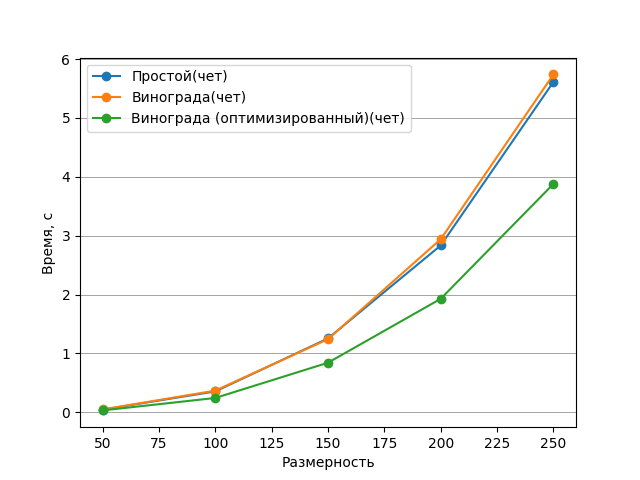
\includegraphics[scale=0.6]{imgs/1.png}
	\caption{Зависимость времени работы алгоритмов при чётных размерах матрицы}
	\label{img:profiling1}
\end{figure}

\begin{figure}[!h]
	\centering
	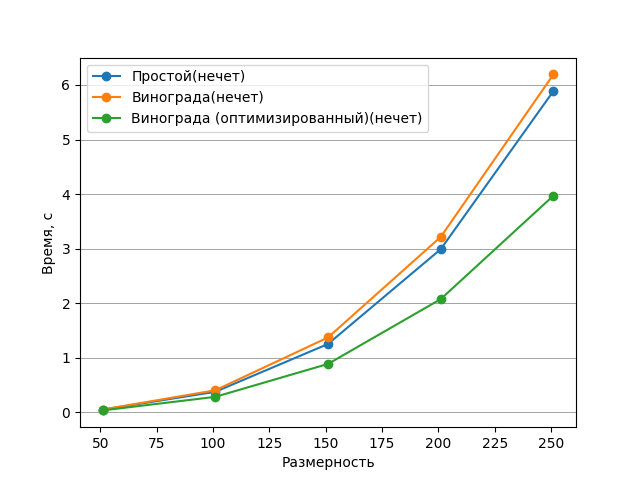
\includegraphics[scale=0.6]{imgs/2.png}
	\caption{Зависимость времени работы алгоритмов при нечётных размерах матрицы}
	\label{img:profiling2}
\end{figure}

\clearpage

\section{Вывод}

Оптимизированный алгоритм Винограда для перемножения матриц работает в $ \approx 1.5 $ раза \textbf{быстрее} классического 
алгоритма перемножения матриц при четных размерностях и $ \approx 1.4 $ раза -- нечетных.
В то же время, неоптимизированный алгоритм Винограда работает в $ \approx 1.03 $ раза \textbf{медленнее} классического 
алгоритма перемножения матриц при четных размерностях и $ \approx 1.07 $ раза -- нечетных.
